%
% teil3.tex -- Beispiel-File für Teil 3
%
% (c) 2020 Prof Dr Andreas Müller, Hochschule Rapperswil
%
% !TEX root = ../../buch.tex
% !TEX encoding = UTF-8
%
\subsection{Initialisierung
\label{genetic_algorithm:initialization}}
Der Startpunkt des genetischen Algorithmus ist die Initialisierung.
Dabei wird eine zufällige Population von möglichen Lösungen erstellt.
Diese wird als ein genetischer String dargestellt.

\begin{figure} [h]
	\centering
	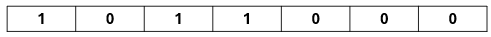
\includegraphics[width=0.8\textwidth]{
        papers/variationsprinzip_algorithmen/images/teil3/01_genetic_string.png
        }
	\caption{Beispiel von möglichen genetischen String}
	\label{fig:possible_genetic_string}
\end{figure}

Dabei wird in jeder Position das Gen aktiviert mit 1 oder deaktiviert mit 0.
Problematik für Stätte funktioniert dies nicht, da wir eine Stadt nicht
einfach aus oder anschalten können. Beim Gen wie oben ändert sich die funktioniert
an der Position nicht. Beispiel Feld 2 ist veranwortlich, dass die Farbe Grün
dargestellt wird. Das ein und auschalten der Städten ist nicht möglich, da sich
es auf die Reihenfolge ankommt. Daher wird wie im nachfolgendem Bild 
\cite{cities_genetic_string}, die jeweilige Nummer der Stadt verwendet.

\begin{figure} [h]
	\centering
	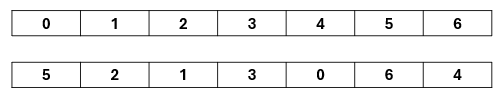
\includegraphics[width=0.8\textwidth]{
        papers/variationsprinzip_algorithmen/images/teil3/02_genetic_string_cities.png
        }
	\caption{Beispiel von Stätten in einem genetischen String dargestellt}
	\label{fig:cities_genetic_string}
\end{figure}

Speziell an der Initialisierung ist, dass man nicht alle Möglichkeiten erstellt,
sondern nur einen kleinen Teil (Population) und damit weiter arbeitet. Diese 
Taktik spart Zeit. 

Die zufällige Erzeugung der Anfangspopulation stellt ebenfalls eine Form der 
Variation dar. Sie sorgt dafür, dass die Suche nicht von einem begrenzten 
Bereich des Lösungsraums startet, sondern eine breite Palette von möglichen 
Lösungen berücksichtigt wird. Dies Bezieht jedoch keine Berechnung mitein,
sondern erstellt zufällige Lösungen und hofft eines kommt nahe an das 
Optimale.
